\documentclass[12pt]{article}

% -------------------- Packages --------------------
\usepackage{hyperref}
\usepackage{listings}
\usepackage[margin=1in]{geometry}
\usepackage{enumitem}
\usepackage{array}
\usepackage{titlesec}
\usepackage{helvet}
\renewcommand{\familydefault}{\sfdefault}

% Math packages
\usepackage{amsmath}     % For math equations
\usepackage{amssymb}     % For advanced math symbols
\usepackage{amsfonts}    % For math fonts
\usepackage{gvv}         % Custom matrix/vector formatting
\usepackage{esint}

% Other packages
\usepackage[utf8]{inputenc}
\usepackage{graphicx}
\usepackage{pgfplots}
\pgfplotsset{compat=1.18}
\usepackage{multirow}
\usepackage{float}
\usepackage{caption}
\usepackage{multicol}

% -------------------- Formatting --------------------
\titleformat{\section}{\bfseries\large}{\thesection.}{1em}{}
\setlength{\parindent}{0pt}
\setlength{\parskip}{6pt}
\renewcommand{\labelenumi}{\alph{enumi})}

% -------------------- Document --------------------
\begin{document}

\newpage
\begin{center}
\textbf{\Large AI25BTECH11034 - SUJAL CHAUHAN }\\
\textbf{4.12.48}
\end{center}

\textbf{Question:}\\
Prove that if a plane has the intercept a,b,c and is at a distance of p units from the origin, then $\frac{1}{a^2}+\frac{1}{b^2}+\frac{1}{c^2}=\frac{1}{p^2}$

\textbf{solution}  
Equation of plane in vector form is given by 
\begin{align}
    \begin{tabular}{|c|c|} \hline
    Point   & Positon vector  \\ \hline
     a    & \myvec{a\\ 0 \\0} \\ \hline
     b    & \myvec{0\\ b \\0} \\ \hline
     c    & \myvec{0\\ 0 \\c} \\ \hline
    \end{tabular}
\end{align}
\begin{align}
    \Vec{n}^T\Vec{P}=d
\end{align}
where $\Vec{n}$ is normal unit vector to the plane and $d$ is the distance of the plane from the origin. \\
Now given plane satisfys the vectors
\begin{align}
    \myvec{a & 0 & 0 \\
           0 & b & 0 \\
           0 & 0 & c}\Vec{n}=\myvec{p\\ p\\p}
\end{align}
Now multiply both side with inverse of the matrix
\begin{align}
    \Vec{n}=\frac{1}{abc}\myvec{{bc}& 0 & 0 \\
           0 &{ac} & 0 \\
           0 & 0 & {ab}}\myvec{p\\ p\\p}
\end{align}
\begin{align}
    \Vec{n}=\myvec{\frac{p}{a}\\ \frac{p}{b}\\ \frac{p}{c}}
\end{align}
Now since $\Vec{n}$ is a unit vector then 
\begin{align}
    \Vec{n}^T\Vec{n}=1
\end{align}
\begin{align}
    \frac{1}{a^2}+\frac{1}{b^2}+\frac{1}{c^2}=\frac{1}{p^2}
\end{align}
\newpage
Checking and Ploting using numerical values of a,b,c
\begin{figure}[h]
    \centering
    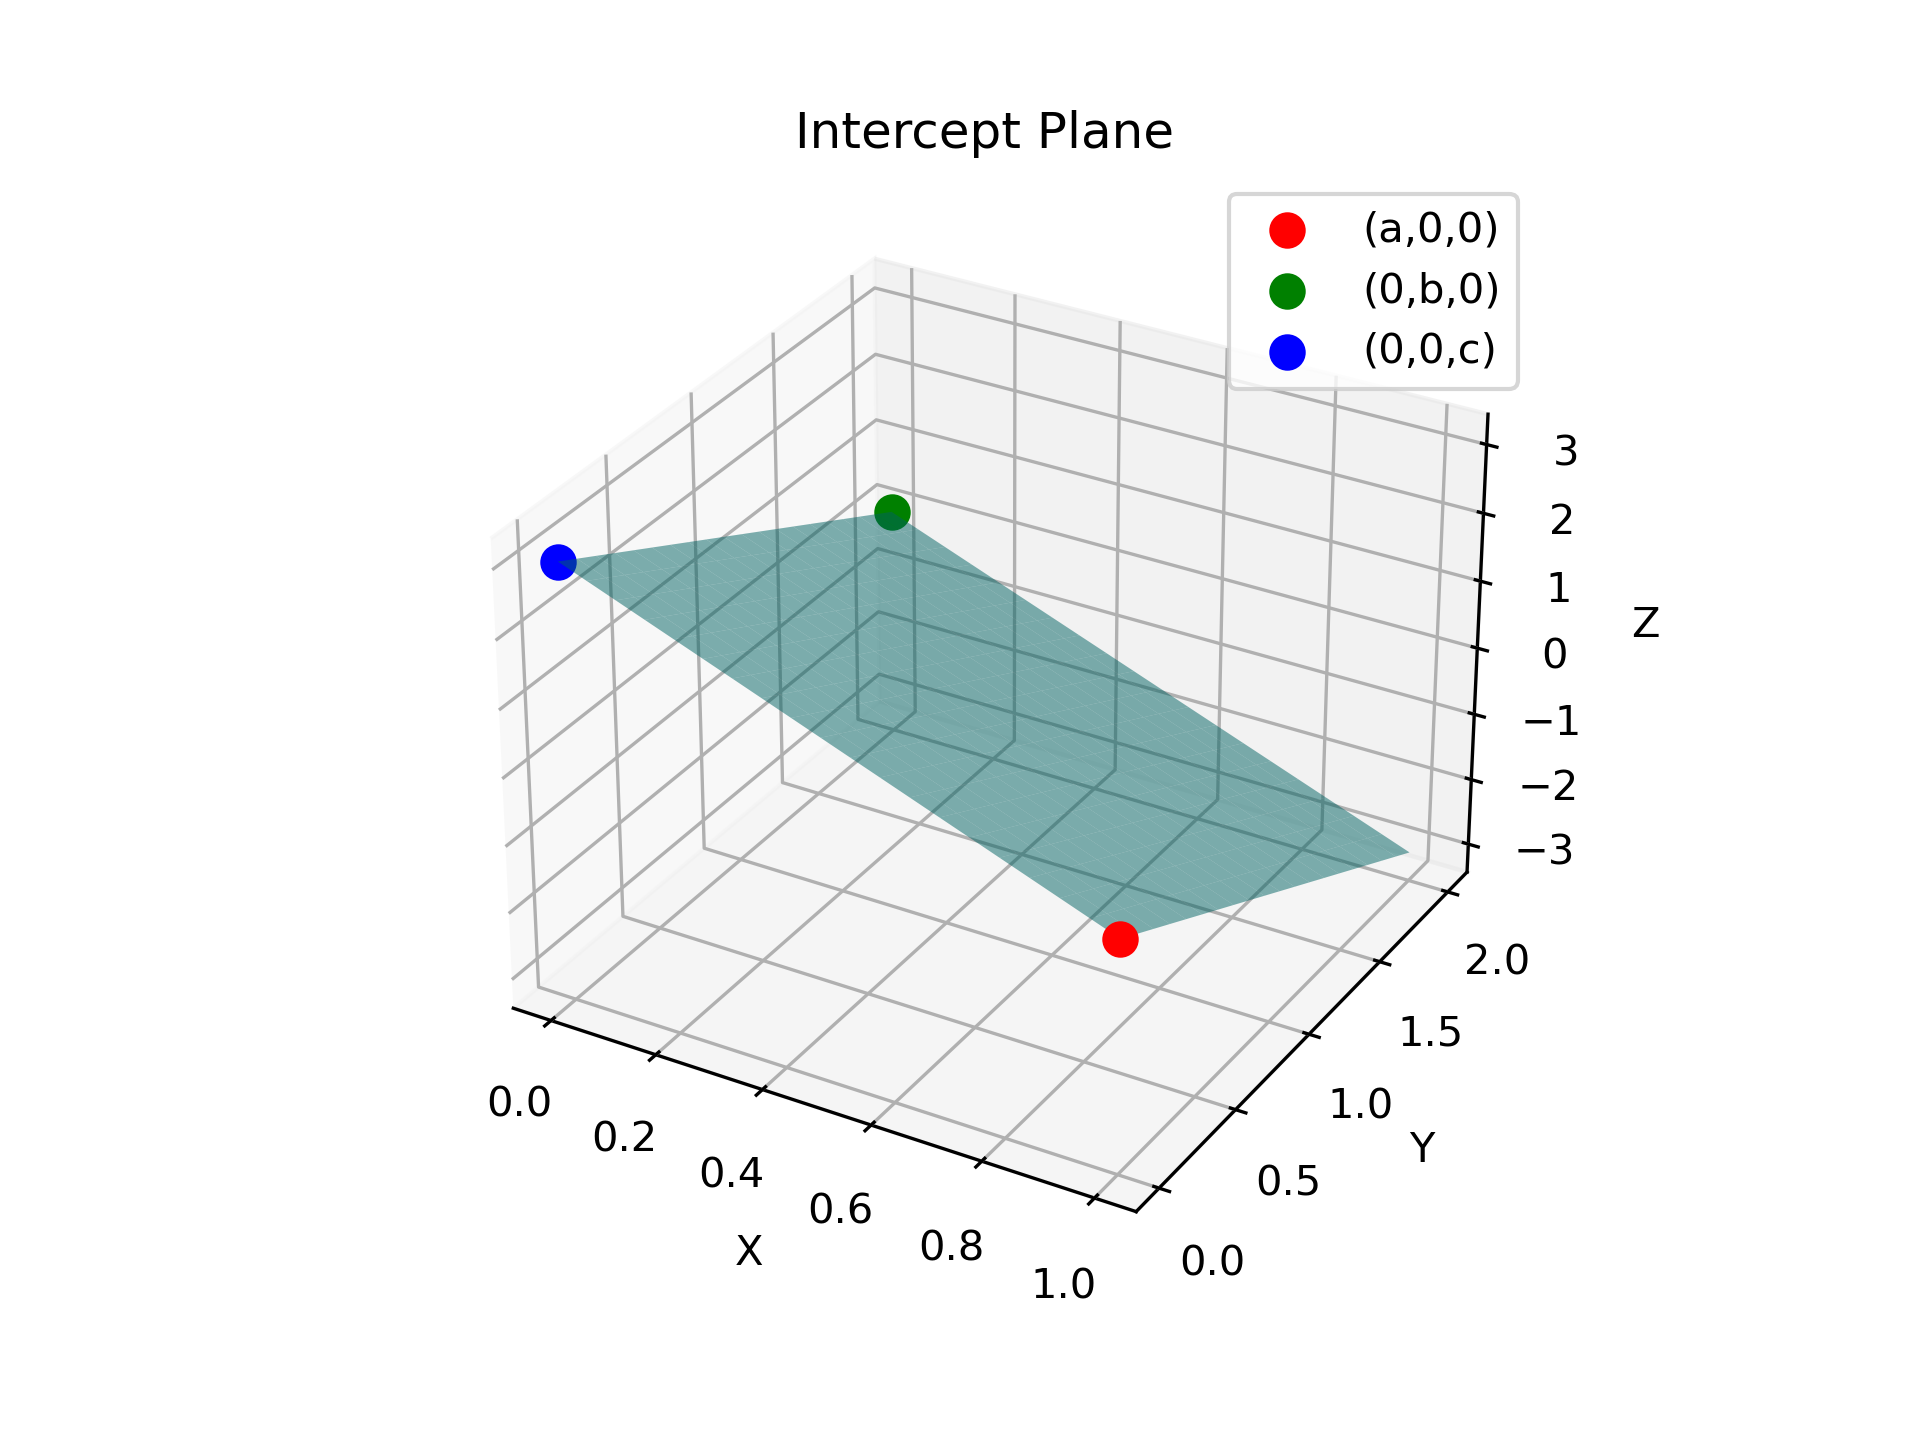
\includegraphics[width=0.5\linewidth]{figures/intercept_plane.png}
    \caption{ploting}
    \label{fig:placeholder}
\end{figure}
\end{document}
